\documentclass[1p]{elsarticle_modified}
%\bibliographystyle{elsarticle-num}

%\usepackage[colorlinks]{hyperref}
%\usepackage{abbrmath_seonhwa} %\Abb, \Ascr, \Acal ,\Abf, \Afrak
\usepackage{amsfonts}
\usepackage{amssymb}
\usepackage{amsmath}
\usepackage{amsthm}
\usepackage{scalefnt}
\usepackage{amsbsy}
\usepackage{kotex}
\usepackage{caption}
\usepackage{subfig}
\usepackage{color}
\usepackage{graphicx}
\usepackage{xcolor} %% white, black, red, green, blue, cyan, magenta, yellow
\usepackage{float}
\usepackage{setspace}
\usepackage{hyperref}

\usepackage{tikz}
\usetikzlibrary{arrows}

\usepackage{multirow}
\usepackage{array} % fixed length table
\usepackage{hhline}

%%%%%%%%%%%%%%%%%%%%%
\makeatletter
\renewcommand*\env@matrix[1][\arraystretch]{%
	\edef\arraystretch{#1}%
	\hskip -\arraycolsep
	\let\@ifnextchar\new@ifnextchar
	\array{*\c@MaxMatrixCols c}}
\makeatother %https://tex.stackexchange.com/questions/14071/how-can-i-increase-the-line-spacing-in-a-matrix
%%%%%%%%%%%%%%%

\usepackage[normalem]{ulem}

\newcommand{\msout}[1]{\ifmmode\text{\sout{\ensuremath{#1}}}\else\sout{#1}\fi}
%SOURCE: \msout is \stkout macro in https://tex.stackexchange.com/questions/20609/strikeout-in-math-mode

\newcommand{\cancel}[1]{
	\ifmmode
	{\color{red}\msout{#1}}
	\else
	{\color{red}\sout{#1}}
	\fi
}

\newcommand{\add}[1]{
	{\color{blue}\uwave{#1}}
}

\newcommand{\replace}[2]{
	\ifmmode
	{\color{red}\msout{#1}}{\color{blue}\uwave{#2}}
	\else
	{\color{red}\sout{#1}}{\color{blue}\uwave{#2}}
	\fi
}

\newcommand{\Sol}{\mathcal{S}} %segment
\newcommand{\D}{D} %diagram
\newcommand{\A}{\mathcal{A}} %arc


%%%%%%%%%%%%%%%%%%%%%%%%%%%%%5 test

\def\sl{\operatorname{\textup{SL}}(2,\Cbb)}
\def\psl{\operatorname{\textup{PSL}}(2,\Cbb)}
\def\quan{\mkern 1mu \triangleright \mkern 1mu}

\theoremstyle{definition}
\newtheorem{thm}{Theorem}[section]
\newtheorem{prop}[thm]{Proposition}
\newtheorem{lem}[thm]{Lemma}
\newtheorem{ques}[thm]{Question}
\newtheorem{cor}[thm]{Corollary}
\newtheorem{defn}[thm]{Definition}
\newtheorem{exam}[thm]{Example}
\newtheorem{rmk}[thm]{Remark}
\newtheorem{alg}[thm]{Algorithm}

\newcommand{\I}{\sqrt{-1}}
\begin{document}

%\begin{frontmatter}
%
%\title{Boundary parabolic representations of knots up to 8 crossings}
%
%%% Group authors per affiliation:
%\author{Yunhi Cho} 
%\address{Department of Mathematics, University of Seoul, Seoul, Korea}
%\ead{yhcho@uos.ac.kr}
%
%
%\author{Seonhwa Kim} %\fnref{s_kim}}
%\address{Center for Geometry and Physics, Institute for Basic Science, Pohang, 37673, Korea}
%\ead{ryeona17@ibs.re.kr}
%
%\author{Hyuk Kim}
%\address{Department of Mathematical Sciences, Seoul National University, Seoul 08826, Korea}
%\ead{hyukkim@snu.ac.kr}
%
%\author{Seokbeom Yoon}
%\address{Department of Mathematical Sciences, Seoul National University, Seoul, 08826,  Korea}
%\ead{sbyoon15@snu.ac.kr}
%
%\begin{abstract}
%We find all boundary parabolic representation of knots up to 8 crossings.
%
%\end{abstract}
%\begin{keyword}
%    \MSC[2010] 57M25 
%\end{keyword}
%
%\end{frontmatter}

%\linenumbers
%\tableofcontents
%
\newcommand\colored[1]{\textcolor{white}{\rule[-0.35ex]{0.8em}{1.4ex}}\kern-0.8em\color{red} #1}%
%\newcommand\colored[1]{\textcolor{white}{ #1}\kern-2.17ex	\textcolor{white}{ #1}\kern-1.81ex	\textcolor{white}{ #1}\kern-2.15ex\color{red}#1	}

{\Large $\underline{11a_{192}~(K11a_{192})}$}

\setlength{\tabcolsep}{10pt}
\renewcommand{\arraystretch}{1.6}
\vspace{1cm}\begin{tabular}{m{100pt}>{\centering\arraybackslash}m{274pt}}
\multirow{5}{120pt}{
	\centering
	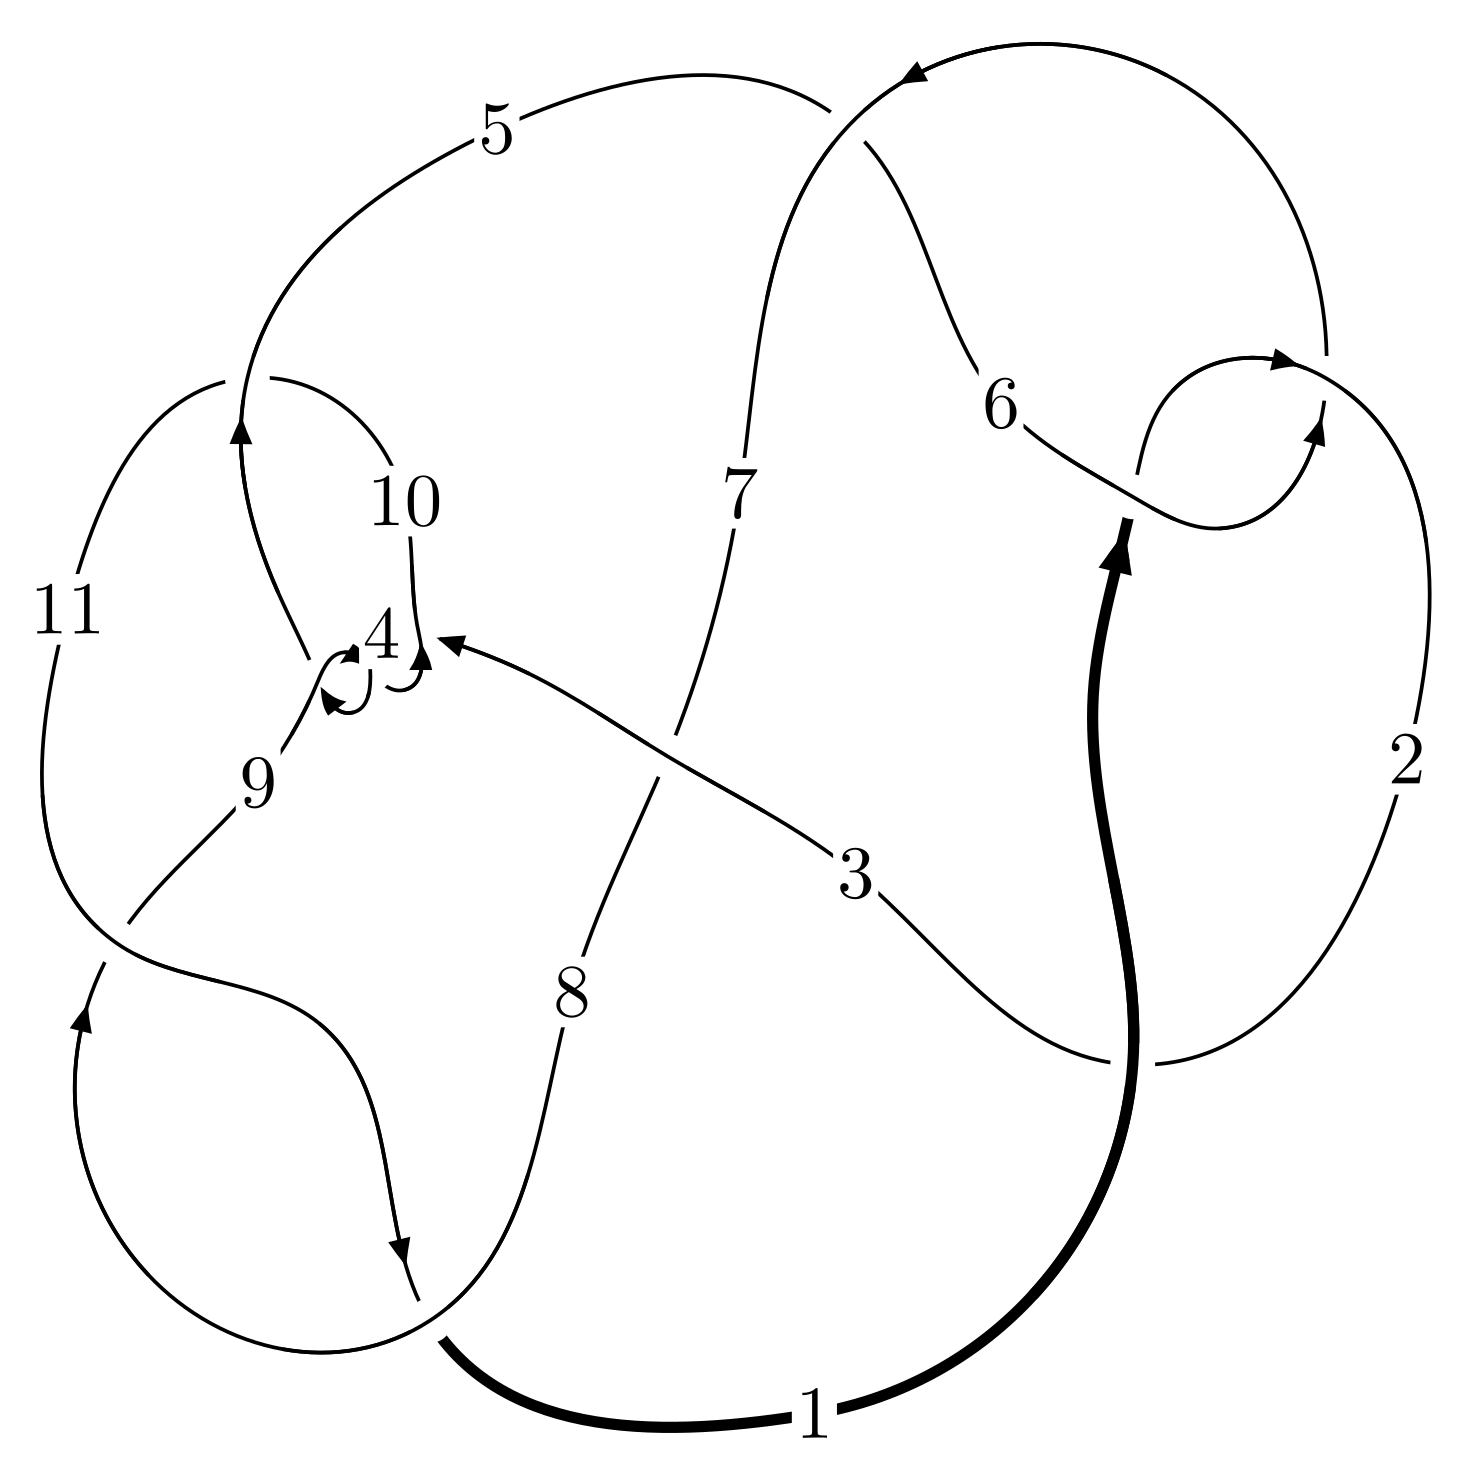
\includegraphics[width=112pt]{../../../GIT/diagram.site/Diagrams/png/441_11a_192.png}\\
\ \ \ A knot diagram\footnotemark}&
\allowdisplaybreaks
\textbf{Linearized knot diagam} \\
\cline{2-2}
 &
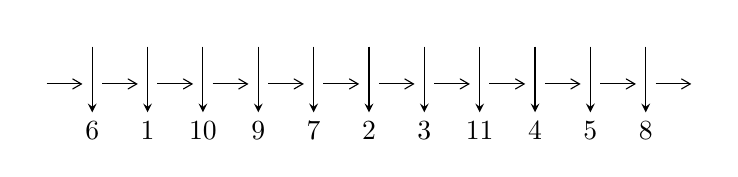
\begin{tikzpicture}[x=20pt, y=17pt]
	% nodes
	\node (C0) at (0, 0) {};
	\node (C1) at (1, 0) {};
	\node (C1U) at (1, +1) {};
	\node (C1D) at (1, -1) {6};

	\node (C2) at (2, 0) {};
	\node (C2U) at (2, +1) {};
	\node (C2D) at (2, -1) {1};

	\node (C3) at (3, 0) {};
	\node (C3U) at (3, +1) {};
	\node (C3D) at (3, -1) {10};

	\node (C4) at (4, 0) {};
	\node (C4U) at (4, +1) {};
	\node (C4D) at (4, -1) {9};

	\node (C5) at (5, 0) {};
	\node (C5U) at (5, +1) {};
	\node (C5D) at (5, -1) {7};

	\node (C6) at (6, 0) {};
	\node (C6U) at (6, +1) {};
	\node (C6D) at (6, -1) {2};

	\node (C7) at (7, 0) {};
	\node (C7U) at (7, +1) {};
	\node (C7D) at (7, -1) {3};

	\node (C8) at (8, 0) {};
	\node (C8U) at (8, +1) {};
	\node (C8D) at (8, -1) {11};

	\node (C9) at (9, 0) {};
	\node (C9U) at (9, +1) {};
	\node (C9D) at (9, -1) {4};

	\node (C10) at (10, 0) {};
	\node (C10U) at (10, +1) {};
	\node (C10D) at (10, -1) {5};

	\node (C11) at (11, 0) {};
	\node (C11U) at (11, +1) {};
	\node (C11D) at (11, -1) {8};
	\node (C12) at (12, 0) {};

	% arrows
	\draw[->,>={angle 60}]
	(C0) edge (C1) (C1) edge (C2) (C2) edge (C3) (C3) edge (C4) (C4) edge (C5) (C5) edge (C6) (C6) edge (C7) (C7) edge (C8) (C8) edge (C9) (C9) edge (C10) (C10) edge (C11) (C11) edge (C12) ;	\draw[->,>=stealth]
	(C1U) edge (C1D) (C2U) edge (C2D) (C3U) edge (C3D) (C4U) edge (C4D) (C5U) edge (C5D) (C6U) edge (C6D) (C7U) edge (C7D) (C8U) edge (C8D) (C9U) edge (C9D) (C10U) edge (C10D) (C11U) edge (C11D) ;
	\end{tikzpicture} \\
\hhline{~~} \\& 
\textbf{Solving Sequence} \\ \cline{2-2} 
 &
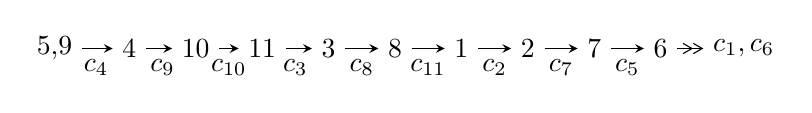
\begin{tikzpicture}[x=24pt, y=7pt]
	% node
	\node (A0) at (-1/8, 0) {5,9};
	\node (A1) at (1, 0) {4};
	\node (A2) at (2, 0) {10};
	\node (A3) at (3, 0) {11};
	\node (A4) at (4, 0) {3};
	\node (A5) at (5, 0) {8};
	\node (A6) at (6, 0) {1};
	\node (A7) at (7, 0) {2};
	\node (A8) at (8, 0) {7};
	\node (A9) at (9, 0) {6};
	\node (C1) at (1/2, -1) {$c_{4}$};
	\node (C2) at (3/2, -1) {$c_{9}$};
	\node (C3) at (5/2, -1) {$c_{10}$};
	\node (C4) at (7/2, -1) {$c_{3}$};
	\node (C5) at (9/2, -1) {$c_{8}$};
	\node (C6) at (11/2, -1) {$c_{11}$};
	\node (C7) at (13/2, -1) {$c_{2}$};
	\node (C8) at (15/2, -1) {$c_{7}$};
	\node (C9) at (17/2, -1) {$c_{5}$};
	\node (A10) at (41/4, 0) {$c_{1},c_{6}$};

	% edge
	\draw[->,>=stealth]	
	(A0) edge (A1) (A1) edge (A2) (A2) edge (A3) (A3) edge (A4) (A4) edge (A5) (A5) edge (A6) (A6) edge (A7) (A7) edge (A8) (A8) edge (A9) ;
	\draw[->>,>={angle 60}]	
	(A9) edge (A10);
\end{tikzpicture} \\ 

\end{tabular} \\

\footnotetext{
The image of knot diagram is generated by the software ``\textbf{Draw programme}" developed by Andrew Bartholomew(\url{http://www.layer8.co.uk/maths/draw/index.htm\#Running-draw}), where we modified some parts for our purpose(\url{https://github.com/CATsTAILs/LinksPainter}).
}\phantom \\ \newline 
\centering \textbf{Ideals for irreducible components\footnotemark of $X_{\text{par}}$} 
 
\begin{align*}
I^u_{1}&=\langle 
u^{48}+u^{47}+\cdots-4 u-1\rangle \\
\\
\end{align*}
\raggedright * 1 irreducible components of $\dim_{\mathbb{C}}=0$, with total 48 representations.\\
\footnotetext{All coefficients of polynomials are rational numbers. But the coefficients are sometimes approximated in decimal forms when there is not enough margin.}
\newpage
\renewcommand{\arraystretch}{1}
\centering \section*{I. $I^u_{1}= \langle u^{48}+u^{47}+\cdots-4 u-1 \rangle$}
\flushleft \textbf{(i) Arc colorings}\\
\begin{tabular}{m{7pt} m{180pt} m{7pt} m{180pt} }
\flushright $a_{5}=$&$\begin{pmatrix}1\\0\end{pmatrix}$ \\
\flushright $a_{9}=$&$\begin{pmatrix}0\\u\end{pmatrix}$ \\
\flushright $a_{4}=$&$\begin{pmatrix}1\\- u^2\end{pmatrix}$ \\
\flushright $a_{10}=$&$\begin{pmatrix}- u\\u^3+u\end{pmatrix}$ \\
\flushright $a_{11}=$&$\begin{pmatrix}- u^3-2 u\\u^3+u\end{pmatrix}$ \\
\flushright $a_{3}=$&$\begin{pmatrix}u^2+1\\- u^4-2 u^2\end{pmatrix}$ \\
\flushright $a_{8}=$&$\begin{pmatrix}u^7+4 u^5+4 u^3\\- u^7-3 u^5-2 u^3+u\end{pmatrix}$ \\
\flushright $a_{1}=$&$\begin{pmatrix}- u^{11}-6 u^9-12 u^7-8 u^5- u^3-2 u\\u^{11}+5 u^9+8 u^7+3 u^5- u^3+u\end{pmatrix}$ \\
\flushright $a_{2}=$&$\begin{pmatrix}- u^{26}-13 u^{24}+\cdots+3 u^2+1\\u^{26}+12 u^{24}+\cdots+4 u^4-3 u^2\end{pmatrix}$ \\
\flushright $a_{7}=$&$\begin{pmatrix}u^{13}+6 u^{11}+13 u^9+12 u^7+6 u^5+4 u^3+u\\- u^{15}-7 u^{13}-18 u^{11}-19 u^9-6 u^7-2 u^5-4 u^3+u\end{pmatrix}$ \\
\flushright $a_{6}=$&$\begin{pmatrix}- u^{28}-13 u^{26}+\cdots+u^2+1\\u^{30}+14 u^{28}+\cdots-8 u^4+u^2\end{pmatrix}$\\ \flushright $a_{6}=$&$\begin{pmatrix}- u^{28}-13 u^{26}+\cdots+u^2+1\\u^{30}+14 u^{28}+\cdots-8 u^4+u^2\end{pmatrix}$\\&\end{tabular}
\flushleft \textbf{(ii) Obstruction class $= -1$}\\~\\
\flushleft \textbf{(iii) Cusp Shapes $= 4 u^{47}+4 u^{46}+\cdots-24 u-22$}\\~\\
\newpage\renewcommand{\arraystretch}{1}
\flushleft \textbf{(iv) u-Polynomials at the component}\newline \\
\begin{tabular}{m{50pt}|m{274pt}}
Crossings & \hspace{64pt}u-Polynomials at each crossing \\
\hline $$\begin{aligned}c_{1},c_{6}\end{aligned}$$&$\begin{aligned}
&u^{48}- u^{47}+\cdots+4 u^2-1
\end{aligned}$\\
\hline $$\begin{aligned}c_{2},c_{5}\end{aligned}$$&$\begin{aligned}
&u^{48}+15 u^{47}+\cdots+8 u+1
\end{aligned}$\\
\hline $$\begin{aligned}c_{3},c_{4},c_{9}\end{aligned}$$&$\begin{aligned}
&u^{48}+u^{47}+\cdots-4 u-1
\end{aligned}$\\
\hline $$\begin{aligned}c_{7}\end{aligned}$$&$\begin{aligned}
&u^{48}+u^{47}+\cdots-282 u-61
\end{aligned}$\\
\hline $$\begin{aligned}c_{8},c_{11}\end{aligned}$$&$\begin{aligned}
&u^{48}-7 u^{47}+\cdots-16 u+1
\end{aligned}$\\
\hline $$\begin{aligned}c_{10}\end{aligned}$$&$\begin{aligned}
&u^{48}- u^{47}+\cdots-198 u-37
\end{aligned}$\\
\hline
\end{tabular}\\~\\
\newpage\renewcommand{\arraystretch}{1}
\flushleft \textbf{(v) Riley Polynomials at the component}\newline \\
\begin{tabular}{m{50pt}|m{274pt}}
Crossings & \hspace{64pt}Riley Polynomials at each crossing \\
\hline $$\begin{aligned}c_{1},c_{6}\end{aligned}$$&$\begin{aligned}
&y^{48}-15 y^{47}+\cdots-8 y+1
\end{aligned}$\\
\hline $$\begin{aligned}c_{2},c_{5}\end{aligned}$$&$\begin{aligned}
&y^{48}+37 y^{47}+\cdots-40 y+1
\end{aligned}$\\
\hline $$\begin{aligned}c_{3},c_{4},c_{9}\end{aligned}$$&$\begin{aligned}
&y^{48}+45 y^{47}+\cdots-8 y+1
\end{aligned}$\\
\hline $$\begin{aligned}c_{7}\end{aligned}$$&$\begin{aligned}
&y^{48}+13 y^{47}+\cdots-22428 y+3721
\end{aligned}$\\
\hline $$\begin{aligned}c_{8},c_{11}\end{aligned}$$&$\begin{aligned}
&y^{48}+41 y^{47}+\cdots+200 y+1
\end{aligned}$\\
\hline $$\begin{aligned}c_{10}\end{aligned}$$&$\begin{aligned}
&y^{48}+17 y^{47}+\cdots+24140 y+1369
\end{aligned}$\\
\hline
\end{tabular}\\~\\
\newpage\flushleft \textbf{(vi) Complex Volumes and Cusp Shapes}
$$\begin{array}{c|c|c}  
\text{Solutions to }I^u_{1}& \I (\text{vol} + \sqrt{-1}CS) & \text{Cusp shape}\\
 \hline 
\begin{aligned}
u &= \phantom{-}0.068968 + 1.151590 I\end{aligned}
 & \phantom{-}2.32852 + 2.32135 I & -10.38591 + 0. I\phantom{ +0.000000I} \\ \hline\begin{aligned}
u &= \phantom{-}0.068968 - 1.151590 I\end{aligned}
 & \phantom{-}2.32852 - 2.32135 I & -10.38591 + 0. I\phantom{ +0.000000I} \\ \hline\begin{aligned}
u &= -0.683357 + 0.405926 I\end{aligned}
 & \phantom{-}5.21260 + 9.77857 I & -8.26482 - 8.48475 I \\ \hline\begin{aligned}
u &= -0.683357 - 0.405926 I\end{aligned}
 & \phantom{-}5.21260 - 9.77857 I & -8.26482 + 8.48475 I \\ \hline\begin{aligned}
u &= \phantom{-}0.673489 + 0.415868 I\end{aligned}
 & \phantom{-}6.02949 - 3.89902 I & -6.63992 + 3.50313 I \\ \hline\begin{aligned}
u &= \phantom{-}0.673489 - 0.415868 I\end{aligned}
 & \phantom{-}6.02949 + 3.89902 I & -6.63992 - 3.50313 I \\ \hline\begin{aligned}
u &= -0.576773 + 0.522352 I\end{aligned}
 & \phantom{-}5.67693 - 5.57732 I & -6.94459 + 2.40000 I \\ \hline\begin{aligned}
u &= -0.576773 - 0.522352 I\end{aligned}
 & \phantom{-}5.67693 + 5.57732 I & -6.94459 - 2.40000 I \\ \hline\begin{aligned}
u &= \phantom{-}0.589475 + 0.506546 I\end{aligned}
 & \phantom{-}6.39491 - 0.29411 I & -5.62712 + 2.80614 I \\ \hline\begin{aligned}
u &= \phantom{-}0.589475 - 0.506546 I\end{aligned}
 & \phantom{-}6.39491 + 0.29411 I & -5.62712 - 2.80614 I \\ \hline\begin{aligned}
u &= \phantom{-}0.173044 + 1.237190 I\end{aligned}
 & -0.64228 - 2.86520 I & \phantom{-0.000000 } 0 \\ \hline\begin{aligned}
u &= \phantom{-}0.173044 - 1.237190 I\end{aligned}
 & -0.64228 + 2.86520 I & \phantom{-0.000000 } 0 \\ \hline\begin{aligned}
u &= -0.640543 + 0.369715 I\end{aligned}
 & -0.68024 + 4.58900 I & -13.6527 - 7.1281 I \\ \hline\begin{aligned}
u &= -0.640543 - 0.369715 I\end{aligned}
 & -0.68024 - 4.58900 I & -13.6527 + 7.1281 I \\ \hline\begin{aligned}
u &= \phantom{-}0.603013 + 0.419142 I\end{aligned}
 & \phantom{-}2.62424 - 1.94253 I & -5.82906 + 3.77516 I \\ \hline\begin{aligned}
u &= \phantom{-}0.603013 - 0.419142 I\end{aligned}
 & \phantom{-}2.62424 + 1.94253 I & -5.82906 - 3.77516 I \\ \hline\begin{aligned}
u &= -0.090373 + 1.285590 I\end{aligned}
 & \phantom{-}3.24763 + 1.60907 I & \phantom{-0.000000 } 0 \\ \hline\begin{aligned}
u &= -0.090373 - 1.285590 I\end{aligned}
 & \phantom{-}3.24763 - 1.60907 I & \phantom{-0.000000 } 0 \\ \hline\begin{aligned}
u &= \phantom{-}0.218506 + 1.294790 I\end{aligned}
 & \phantom{-}3.84600 - 8.17225 I & \phantom{-0.000000 } 0 \\ \hline\begin{aligned}
u &= \phantom{-}0.218506 - 1.294790 I\end{aligned}
 & \phantom{-}3.84600 + 8.17225 I & \phantom{-0.000000 } 0 \\ \hline\begin{aligned}
u &= -0.505212 + 0.440988 I\end{aligned}
 & -0.223689 - 0.846659 I & -12.11040 + 0.46472 I \\ \hline\begin{aligned}
u &= -0.505212 - 0.440988 I\end{aligned}
 & -0.223689 + 0.846659 I & -12.11040 - 0.46472 I \\ \hline\begin{aligned}
u &= -0.196581 + 1.315430 I\end{aligned}
 & \phantom{-}4.69521 + 2.82559 I & \phantom{-0.000000 } 0 \\ \hline\begin{aligned}
u &= -0.196581 - 1.315430 I\end{aligned}
 & \phantom{-}4.69521 - 2.82559 I & \phantom{-0.000000 } 0 \\ \hline\begin{aligned}
u &= \phantom{-}0.627758 + 0.108061 I\end{aligned}
 & -0.50327 - 5.09371 I & -14.3561 + 6.8355 I \\ \hline\begin{aligned}
u &= \phantom{-}0.627758 - 0.108061 I\end{aligned}
 & -0.50327 + 5.09371 I & -14.3561 - 6.8355 I \\ \hline\begin{aligned}
u &= \phantom{-}0.609769\phantom{ +0.000000I}\end{aligned}
 & -4.36789\phantom{ +0.000000I} & -20.8280\phantom{ +0.000000I} \\ \hline\begin{aligned}
u &= -0.582317 + 0.152321 I\end{aligned}
 & \phantom{-}0.1388920 - 0.0056976 I & -12.76408 - 1.77198 I \\ \hline\begin{aligned}
u &= -0.582317 - 0.152321 I\end{aligned}
 & \phantom{-}0.1388920 + 0.0056976 I & -12.76408 + 1.77198 I \\ \hline\begin{aligned}
u &= -0.012644 + 1.408660 I\end{aligned}
 & \phantom{-}7.96823 + 2.83806 I & \phantom{-0.000000 } 0\\
 \hline 
 \end{array}$$\newpage$$\begin{array}{c|c|c}  
\text{Solutions to }I^u_{1}& \I (\text{vol} + \sqrt{-1}CS) & \text{Cusp shape}\\
 \hline 
\begin{aligned}
u &= -0.012644 - 1.408660 I\end{aligned}
 & \phantom{-}7.96823 - 2.83806 I & \phantom{-0.000000 } 0 \\ \hline\begin{aligned}
u &= -0.074086 + 0.558977 I\end{aligned}
 & \phantom{-}2.01219 + 2.59814 I & -6.70685 - 3.63850 I \\ \hline\begin{aligned}
u &= -0.074086 - 0.558977 I\end{aligned}
 & \phantom{-}2.01219 - 2.59814 I & -6.70685 + 3.63850 I \\ \hline\begin{aligned}
u &= -0.20167 + 1.44404 I\end{aligned}
 & \phantom{-}5.75150 + 1.80433 I & \phantom{-0.000000 } 0 \\ \hline\begin{aligned}
u &= -0.20167 - 1.44404 I\end{aligned}
 & \phantom{-}5.75150 - 1.80433 I & \phantom{-0.000000 } 0 \\ \hline\begin{aligned}
u &= -0.24122 + 1.44657 I\end{aligned}
 & \phantom{-}5.16114 + 7.81947 I & \phantom{-0.000000 } 0 \\ \hline\begin{aligned}
u &= -0.24122 - 1.44657 I\end{aligned}
 & \phantom{-}5.16114 - 7.81947 I & \phantom{-0.000000 } 0 \\ \hline\begin{aligned}
u &= \phantom{-}0.22417 + 1.45752 I\end{aligned}
 & \phantom{-}8.65974 - 4.98357 I & \phantom{-0.000000 } 0 \\ \hline\begin{aligned}
u &= \phantom{-}0.22417 - 1.45752 I\end{aligned}
 & \phantom{-}8.65974 + 4.98357 I & \phantom{-0.000000 } 0 \\ \hline\begin{aligned}
u &= -0.25363 + 1.46457 I\end{aligned}
 & \phantom{-}11.2407 + 13.2008 I & \phantom{-0.000000 } 0 \\ \hline\begin{aligned}
u &= -0.25363 - 1.46457 I\end{aligned}
 & \phantom{-}11.2407 - 13.2008 I & \phantom{-0.000000 } 0 \\ \hline\begin{aligned}
u &= \phantom{-}0.24833 + 1.46680 I\end{aligned}
 & \phantom{-}12.09980 - 7.26678 I & \phantom{-0.000000 } 0 \\ \hline\begin{aligned}
u &= \phantom{-}0.24833 - 1.46680 I\end{aligned}
 & \phantom{-}12.09980 + 7.26678 I & \phantom{-0.000000 } 0 \\ \hline\begin{aligned}
u &= -0.19351 + 1.48062 I\end{aligned}
 & \phantom{-}12.14030 - 2.80062 I & \phantom{-0.000000 } 0 \\ \hline\begin{aligned}
u &= -0.19351 - 1.48062 I\end{aligned}
 & \phantom{-}12.14030 + 2.80062 I & \phantom{-0.000000 } 0 \\ \hline\begin{aligned}
u &= \phantom{-}0.20123 + 1.47969 I\end{aligned}
 & \phantom{-}12.80670 - 3.15758 I & \phantom{-0.000000 } 0 \\ \hline\begin{aligned}
u &= \phantom{-}0.20123 - 1.47969 I\end{aligned}
 & \phantom{-}12.80670 + 3.15758 I & \phantom{-0.000000 } 0 \\ \hline\begin{aligned}
u &= -0.361931\phantom{ +0.000000I}\end{aligned}
 & -0.601903\phantom{ +0.000000I} & -16.4760\phantom{ +0.000000I}\\
 \hline 
 \end{array}$$\newpage
\newpage\renewcommand{\arraystretch}{1}
\centering \section*{ II. u-Polynomials}
\begin{tabular}{m{50pt}|m{274pt}}
Crossings & \hspace{64pt}u-Polynomials at each crossing \\
\hline $$\begin{aligned}c_{1},c_{6}\end{aligned}$$&$\begin{aligned}
&u^{48}- u^{47}+\cdots+4 u^2-1
\end{aligned}$\\
\hline $$\begin{aligned}c_{2},c_{5}\end{aligned}$$&$\begin{aligned}
&u^{48}+15 u^{47}+\cdots+8 u+1
\end{aligned}$\\
\hline $$\begin{aligned}c_{3},c_{4},c_{9}\end{aligned}$$&$\begin{aligned}
&u^{48}+u^{47}+\cdots-4 u-1
\end{aligned}$\\
\hline $$\begin{aligned}c_{7}\end{aligned}$$&$\begin{aligned}
&u^{48}+u^{47}+\cdots-282 u-61
\end{aligned}$\\
\hline $$\begin{aligned}c_{8},c_{11}\end{aligned}$$&$\begin{aligned}
&u^{48}-7 u^{47}+\cdots-16 u+1
\end{aligned}$\\
\hline $$\begin{aligned}c_{10}\end{aligned}$$&$\begin{aligned}
&u^{48}- u^{47}+\cdots-198 u-37
\end{aligned}$\\
\hline
\end{tabular}\newpage\renewcommand{\arraystretch}{1}
\centering \section*{ III. Riley Polynomials}
\begin{tabular}{m{50pt}|m{274pt}}
Crossings & \hspace{64pt}Riley Polynomials at each crossing \\
\hline $$\begin{aligned}c_{1},c_{6}\end{aligned}$$&$\begin{aligned}
&y^{48}-15 y^{47}+\cdots-8 y+1
\end{aligned}$\\
\hline $$\begin{aligned}c_{2},c_{5}\end{aligned}$$&$\begin{aligned}
&y^{48}+37 y^{47}+\cdots-40 y+1
\end{aligned}$\\
\hline $$\begin{aligned}c_{3},c_{4},c_{9}\end{aligned}$$&$\begin{aligned}
&y^{48}+45 y^{47}+\cdots-8 y+1
\end{aligned}$\\
\hline $$\begin{aligned}c_{7}\end{aligned}$$&$\begin{aligned}
&y^{48}+13 y^{47}+\cdots-22428 y+3721
\end{aligned}$\\
\hline $$\begin{aligned}c_{8},c_{11}\end{aligned}$$&$\begin{aligned}
&y^{48}+41 y^{47}+\cdots+200 y+1
\end{aligned}$\\
\hline $$\begin{aligned}c_{10}\end{aligned}$$&$\begin{aligned}
&y^{48}+17 y^{47}+\cdots+24140 y+1369
\end{aligned}$\\
\hline
\end{tabular}
\vskip 2pc
\end{document}